\section{建模结果数据}

\begin{table}[htbp]
\centering
\caption{计算出的数值结果}
\label{table:values}
\begin{tabular}{@{}lll@{}}
\toprule
符号          & 值     &   说明         \\ \midrule
$l$    & $0.2766\,\si{mm}$     & 两个相邻接收器间的距离                  \\
$(x_0, y_0)$ & $(-9.2383\,\si{mm}, 6.2663\,\si{mm})$  & $xoy$坐标系中探测系统旋转中心坐标 \\ \bottomrule
\end{tabular}
\end{table} 

\begin{longtable}{@{}cccccc@{}}
\caption{180个旋转方向}
\label{table:roration_degrees}
\endfirsthead
\endhead
\hline
$29.6422^\circ$ & $30.9957^\circ$ & $31.5511^\circ$ & $32.6404^\circ$ & $33.6726^\circ$ & $34.6418^\circ$\\ \hline
$35.6417^\circ$ & $36.6416^\circ$ & $37.6415^\circ$ & $38.6414^\circ$ & $39.6412^\circ$ & $40.6411^\circ$\\ \hline
$41.6410^\circ$ & $42.6409^\circ$ & $43.6408^\circ$ & $44.7911^\circ$ & $45.6406^\circ$ & $46.6406^\circ$\\ \hline
$47.6405^\circ$ & $48.6404^\circ$ & $49.6403^\circ$ & $50.6402^\circ$ & $51.6402^\circ$ & $52.6400^\circ$\\ \hline
$53.6399^\circ$ & $54.6396^\circ$ & $55.6393^\circ$ & $56.6389^\circ$ & $57.6386^\circ$ & $58.6382^\circ$\\ \hline
$59.6379^\circ$ & $60.5365^\circ$ & $61.6370^\circ$ & $62.6364^\circ$ & $63.6360^\circ$ & $64.6353^\circ$\\ \hline
$65.6349^\circ$ & $66.6342^\circ$ & $67.6335^\circ$ & $68.6327^\circ$ & $69.6320^\circ$ & $70.6309^\circ$\\ \hline
$71.6300^\circ$ & $72.6288^\circ$ & $73.6276^\circ$ & $74.6262^\circ$ & $75.6247^\circ$ & $76.6228^\circ$\\ \hline
$77.6208^\circ$ & $78.6183^\circ$ & $79.6154^\circ$ & $80.6119^\circ$ & $81.6075^\circ$ & $82.6019^\circ$\\ \hline
$83.5949^\circ$ & $84.5856^\circ$ & $85.5718^\circ$ & $86.5496^\circ$ & $87.5109^\circ$ & $88.4265^\circ$\\ \hline
$89.1500^\circ$ & $91.0183^\circ$ & $91.8326^\circ$ & $92.7671^\circ$ & $93.7351^\circ$ & $94.7164^\circ$\\ \hline
$95.7041^\circ$ & $96.6950^\circ$ & $97.6888^\circ$ & $98.6838^\circ$ & $99.6795^\circ$ & $100.6763^\circ$\\ \hline
$101.6735^\circ$ & $102.6712^\circ$ & $103.6692^\circ$ & $104.6676^\circ$ & $105.6659^\circ$ & $106.6646^\circ$\\ \hline
$107.6633^\circ$ & $108.6624^\circ$ & $109.6613^\circ$ & $110.6606^\circ$ & $111.6595^\circ$ & $112.6588^\circ$\\ \hline
$113.6582^\circ$ & $114.6575^\circ$ & $115.6570^\circ$ & $116.6564^\circ$ & $117.4534^\circ$ & $118.6554^\circ$\\ \hline
$119.6549^\circ$ & $120.6546^\circ$ & $121.6543^\circ$ & $122.6538^\circ$ & $123.6535^\circ$ & $124.6532^\circ$\\ \hline
$125.6529^\circ$ & $126.6526^\circ$ & $127.6524^\circ$ & $128.6523^\circ$ & $129.6521^\circ$ & $130.6521^\circ$\\ \hline
$131.7520^\circ$ & $132.6519^\circ$ & $133.6519^\circ$ & $134.6518^\circ$ & $135.6517^\circ$ & $136.6517^\circ$\\ \hline
$137.6516^\circ$ & $138.6515^\circ$ & $139.6514^\circ$ & $140.6513^\circ$ & $141.6511^\circ$ & $142.6510^\circ$\\ \hline
$143.6509^\circ$ & $144.6508^\circ$ & $145.6507^\circ$ & $146.6507^\circ$ & $147.6505^\circ$ & $148.6505^\circ$\\ \hline
$149.6504^\circ$ & $150.6503^\circ$ & $151.6502^\circ$ & $152.6502^\circ$ & $153.6501^\circ$ & $154.6501^\circ$\\ \hline
$155.6501^\circ$ & $156.6500^\circ$ & $157.6500^\circ$ & $158.6500^\circ$ & $159.6500^\circ$ & $160.6500^\circ$\\ \hline
$161.6500^\circ$ & $162.6500^\circ$ & $163.6501^\circ$ & $164.6501^\circ$ & $165.6503^\circ$ & $166.6503^\circ$\\ \hline
$167.6506^\circ$ & $168.6508^\circ$ & $169.6510^\circ$ & $170.6513^\circ$ & $171.6517^\circ$ & $172.6523^\circ$\\ \hline
$173.6530^\circ$ & $174.6541^\circ$ & $175.6556^\circ$ & $176.6584^\circ$ & $177.6633^\circ$ & $178.6757^\circ$\\ \hline
$179.7497^\circ$ & $180.5807^\circ$ & $181.6219^\circ$ & $182.6311^\circ$ & $183.6351^\circ$ & $184.6373^\circ$\\ \hline
$185.6387^\circ$ & $186.6397^\circ$ & $187.6404^\circ$ & $188.6409^\circ$ & $189.6413^\circ$ & $190.6416^\circ$\\ \hline
$191.6419^\circ$ & $192.6421^\circ$ & $193.6422^\circ$ & $194.6423^\circ$ & $195.6424^\circ$ & $196.6425^\circ$\\ \hline
$197.6425^\circ$ & $198.6425^\circ$ & $199.6425^\circ$ & $200.6425^\circ$ & $201.6425^\circ$ & $202.6425^\circ$\\ \hline
$203.6425^\circ$ & $204.6424^\circ$ & $205.6424^\circ$ & $206.6424^\circ$ & $207.6423^\circ$ & $208.6317^\circ$\\ \hline
\end{longtable}

\begin{figure}[htbp]
  \centering
  \begin{subfigure}[b]{0.3\textwidth}
    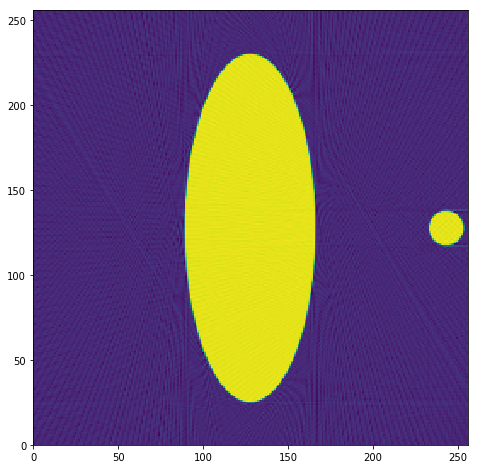
\includegraphics[width=\linewidth]{2_filter_2.png}
    \caption{附件(2)}
  \end{subfigure}%
  \hfill
  \begin{subfigure}[b]{0.3\textwidth}
    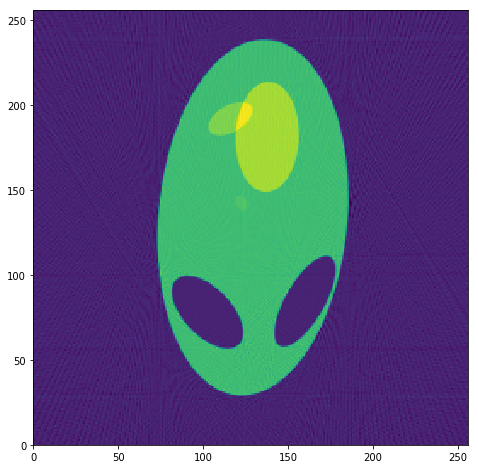
\includegraphics[width=\linewidth]{2_filter_3.png}
    \caption{附件(3)}
  \end{subfigure}%
  \hfill
  \begin{subfigure}[b]{0.3\textwidth}
    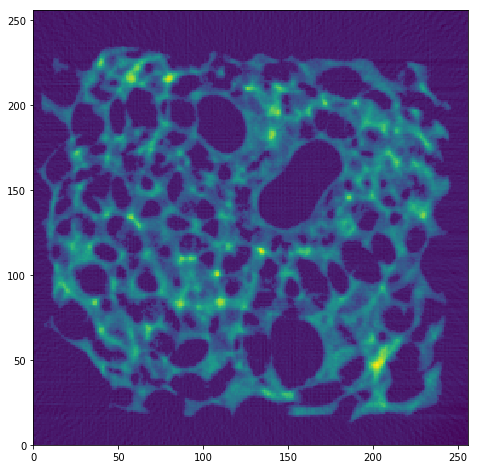
\includegraphics[width=\linewidth]{2_filter_5.png}
    \caption{附件(5)}
  \end{subfigure}
  \caption{滤波反投影恢复出的介质}
  \label{fig:4_filter_copy}
\end{figure}

\begin{table}[htbp]
\centering
\caption{两样例给定点处的吸收率数据}
\label{table:absort_rate}
\begin{tabular}{@{}cccccc@{}}
\toprule
      & 1         & 2        & 3         & 4        & 5  \\ \midrule	
附件(3) & $0$ & $0.9979$ & $0$ & $1.2050$ & $1.0866$ \\
附件(5) & $0.0780$  & $2.8227$ & $6.7965$  & $0.1994$ & $0.1626$ \\ \bottomrule
      & 6         & 7        & 8         & 9        & 10  \\ \midrule
附件(3)& $1.4175$ & $1.2915$ & $0.0064$  & $0.0286$ & $0$ \\
附件(5)& $3.1407$ & $6.4676$ & $0$ & $7.3136$ & $0$ \\ \bottomrule
\end{tabular}
\end{table}